%
%===============>>  Киселев Модуль 7 <<=============
%
\setmodule{7}

%BEGIN_FOLD % ====>>_____ Занятие 1 _____<<====
\begin{class}[number=1]
	\begin{listofex}
		\item .
	\end{listofex}
\end{class}
%END_FOLD

%BEGIN_FOLD % ====>>_____ Занятие 2 _____<<====
\begin{class}[number=2]
	\begin{listofex}
		\item .
	\end{listofex}
\end{class}
%END_FOLD

%BEGIN_FOLD % ====>>_ Домашняя работа 1 _<<====
\begin{homework}[number=1]
	\begin{listofex}
		\item .
	\end{listofex}
\end{homework}
%END_FOLD

%BEGIN_FOLD % ====>>_____ Занятие 3 _____<<====
\begin{class}[number=3]
		\begin{definit}
		\textbf{Синусом} острого угла прямоугольного треугольника называется отношение противолежащего катета к гипотенузе.
		\end{definit}
		\begin{definit}
		\textbf{Косинусом} острого угла прямоугольного треугольника называется отношение прилежащего катета к гипотенузе.
		\end{definit}
		\begin{definit}
		\textbf{Тангенсом} острого угла прямоугольного треугольника называется отношение противолежащего катета к прилежащему катету.
		\end{definit}
		\begin{definit}
		\textbf{Основное тригонометрическое тождество:} \[\sin^2\alpha+\cos^2\alpha=1\]
		\end{definit}
		\begin{listofex}
		\item В треугольнике \( ABC \) угол \( C \) равен \( 90 \) градусов, \( AC=6 \), \( AB=20 \). Найдите \( \sin B \).
		\item  В треугольнике \( ABC \) угол \( C \) равен \( 90 \) градусов, \( BC=9 \), \( AB=20 \). Найдите \( \cos B \).
		\item В треугольнике \( ABC \) угол \( C \) равен \( 90 \) градусов, \( BC=9 \), \( AC=27 \). Найдите \( \tg B \).
		\item Найдите синус, косинус и тангенс углов \( A \) и \( B \) треугольника \( ABC \) с прямым углом \( C \), если:
		\begin{tasks}(2)
			\task \( BC=8 \), \( AB=17 \)
			\task \( BC=21 \), \( AC=20 \)
			\task \( BC=1 \), \( AC=2 \)
		\end{tasks}
		\item Найдите:
		\begin{tasks}(1)
			\task \( \sin\alpha \) и \( \tg\alpha \), если \( \cos\alpha=\dfrac{1}{2} \)
			\task \( \cos\alpha \) и \( \tg\alpha \), если \( \sin\alpha=\dfrac{\sqrt{3}}{2} \)
		\end{tasks}
		\item В треугольнике \( ABC \) угол \( C \) прямой, \( BC=8 \), \( \sin A=0,4 \). Найдите \( AB \).
		\item В треугольнике \( ABC \) угол \( C \) прямой, \( AC=15 \), \( \cos A=\dfrac{5}{7} \). Найдите \( AB \).
		\item В треугольнике \( ABC \) угол \( C \) равен \( 90\degree \), \( BC=12 \), \( \sin A=\dfrac{4}{11} \). Найдите \( AB \).
		\item В треугольнике \( ABC \) угол \( C \) равен \( 90\degree \), \( AC = 4,8 \),  \( \sin A = \dfrac{7}{25} \).  Найдите \( AB \).
		\item В треугольнике \( ABC \) угол \( C \) равен \( 90\degree \),  \( \tg A = \dfrac{33}{4\sqrt{33}} \),  \( AC =  4 \). Найдите \( AB \).
		\item В треугольнике \( АВС \) угол \( С \) равен \( 90\degree \), высота \( CH \) равна \( 7 \), \( BH = 24 \). Найдите  \( \cos A \).
		\item В треугольнике \( ABC \) \( AC=BC=5\),  \( \sin A = \dfrac{7}{25} \).  Найдите \(AB\).
		\item В треугольнике \( ABC \) \( AC = BC = 8 \),  \( \cos A = 0,5 \). Найдите \(AB\).
		\item В треугольнике \( ABC \) угол \( C \) равен \( 90\degree \), \( BC=5 \), \( \sin A=\dfrac{7}{25} \).  Найдите высоту \( CH \).
		\item В треугольнике \( ABC \) угол \( C \) равен \( 90\degree \), \( CH \) --- высота, \( BC=3 \), \( \cos A=\dfrac{\sqrt{35}}{6} \).  Найдите \( AH \).
		\item В треугольнике \( ABC \) угол \( C \) равен \( 90\degree \), \( CH \) --- высота, \( BC=5 \),  \( \cos A=\dfrac{7}{25} \).  Найдите \( BH \).
		\item В треугольнике \( ABC \) \( AC = BC \), \( AH \) --- высота, \( AB = 8 \),  \( \cos BAC = 0,5 \). Найдите \( BH \).
	\end{listofex}
\end{class}
%END_FOLD

%BEGIN_FOLD % ====>>_____ Занятие 4 _____<<====
\begin{class}[number=4]
	\begin{listofex}
		\item .
	\end{listofex}
\end{class}
%END_FOLD

%BEGIN_FOLD % ====>>_ Домашняя работа 2 _<<====
\begin{homework}[number=2]
	\begin{listofex}
		\item В треугольнике \( ABC \) угол \( C \) равен \( 90\degree \), \( BC=6 \), \( \sin A=0,3 \). Найдите \( AB \).
		\item Катеты прямоугольного треугольника равны  \( \sqrt{21} \) и \( 2 \). Найдите синус наименьшего угла этого треугольника.
		\item В треугольнике \( ABC \) угол \( C \) равен \( 90\degree \), \( \tg A=\dfrac{2\sqrt{10}}{3} \),  \( AB=28 \). Найдите \( AC \).
		\item В треугольнике \( ABC \) угол \( C \) равен \( 90\degree \), \( AC=24 \), \( BC=7 \). Найдите \( \sin A \).
		\item В треугольнике \( ABC \) угол \( C \) равен \( 90 \) градусов, \( BC=15 \), \( \cos A=\dfrac{12}{13} \).  Найдите \( AC \).
		\item В треугольнике \( ABC \) угол \( C \) равен \( 156\degree \), \( AC=BC \). Найдите угол \( A \). Ответ дайте в градусах.
		\item В треугольнике \( ABC \) угол \( A \) равен \( 30\degree \), угол \( B \) --- тупой, \( CH \) --- высота, \( \angle BCH=22\degree \). Найдите угол \( ACB \). Ответ дайте в градусах.
	\end{listofex}
\end{homework}
%END_FOLD

%BEGIN_FOLD % ====>>_____ Занятие 5-6 _____<<====
\begin{class}[number=5-6]
	\begin{definit}
	Если секущая пересекает две параллельные прямые, то:
	\begin{tasks}(1)
		\task внутренние накрест лежащие углы равны: \( \angle 4 \) и \( \angle5 \), \( \angle 3 \) и \( \angle 6\);
		\task сумма внутренних односторонних углов равна  \(180\degree\): \( \angle 3 \) и \( \angle 5 \), \( \angle 4 \) и \( \angle 6 \);
		\task соответственные углы равны: \( \angle 1 \) и \( \angle 5 \), \( \angle 2 \) и \( \angle 6 \), \( \angle 3 \) и \( \angle 7 \), \( \angle 4 \) и \( \angle 8 \);
		\task внешние накрест лежащие углы равны: \( \angle 2 \) и \( \angle 7 \), \( \angle 1 \) и \( \angle 8 \);
		\task сумма внешних односторонних углов равна  \(180\degree\): \( \angle 1 \) и \( \angle 7 \), \( \angle 2 \) и \( \angle 8 \).
	\end{tasks}
	\begin{minipage}[c]{0.9\linewidth}
		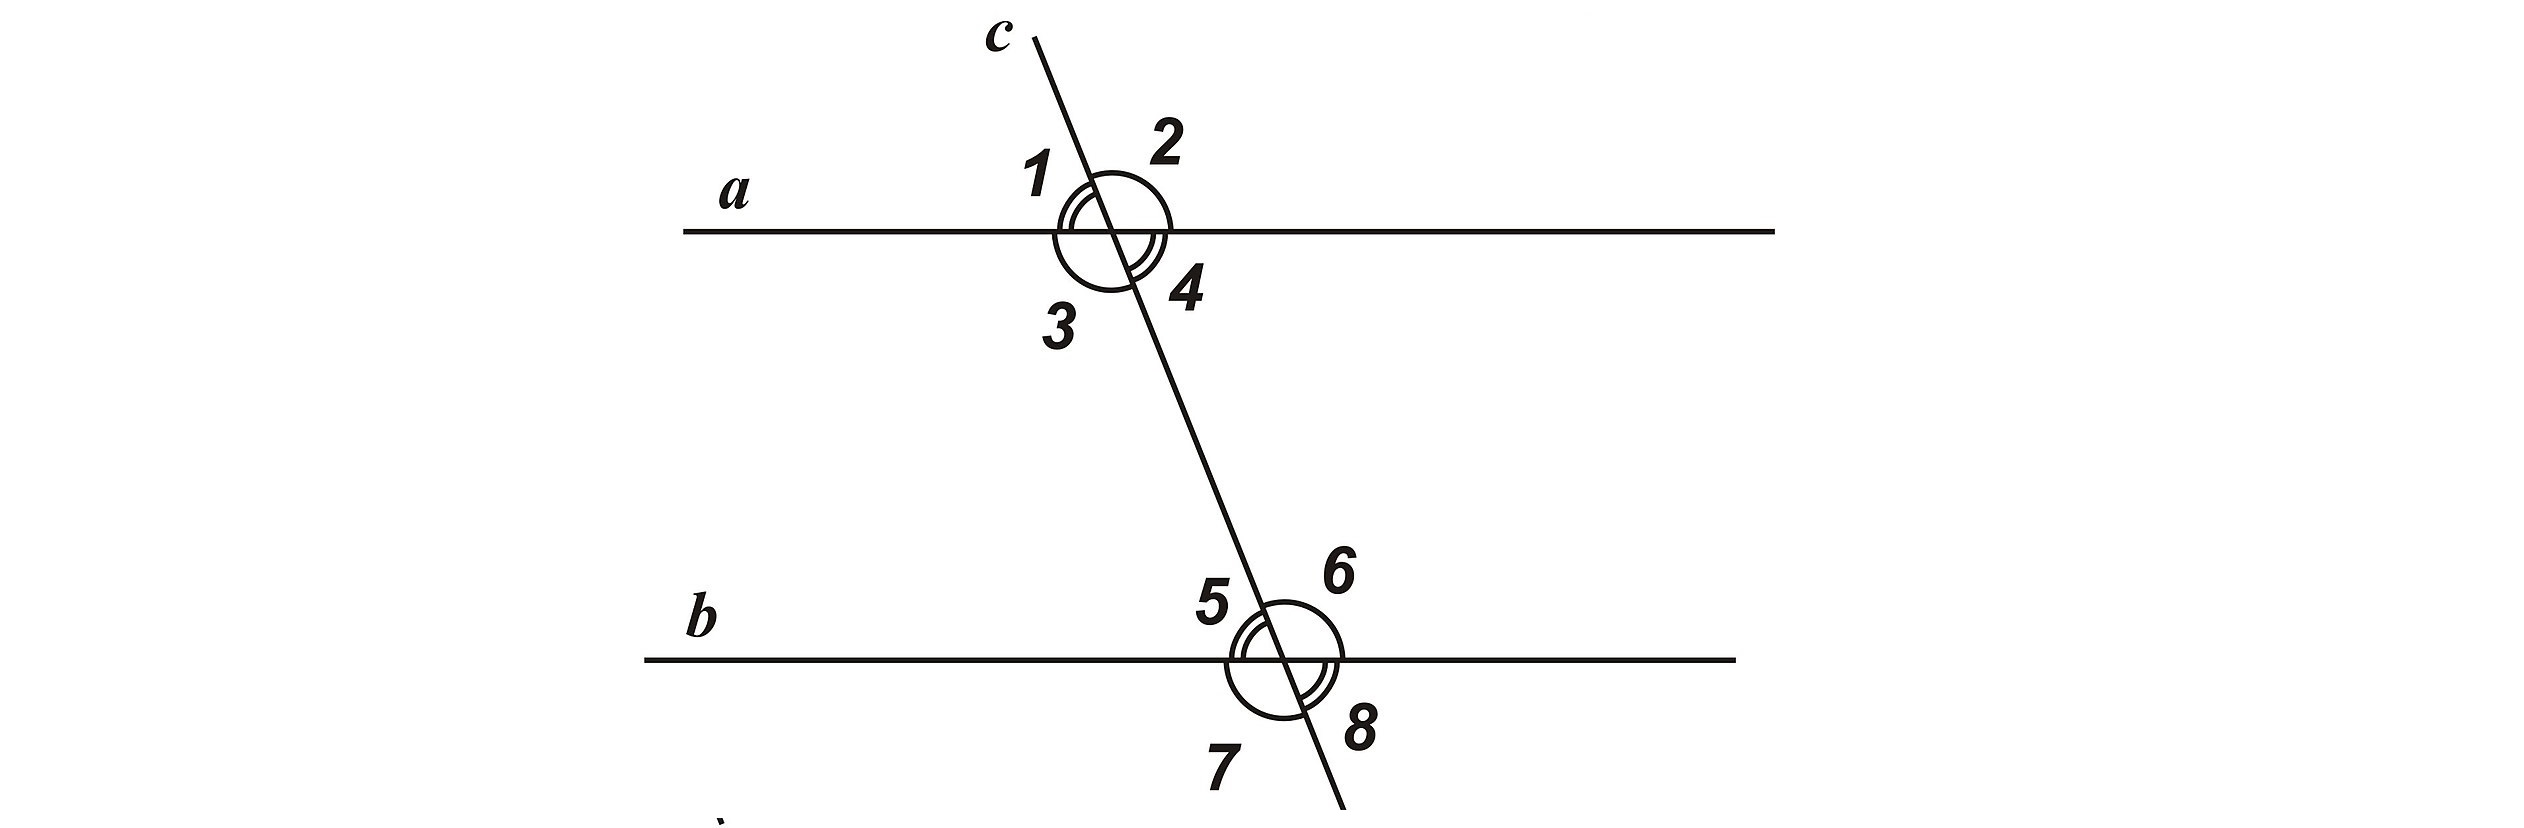
\includegraphics[align=t, width=\linewidth]{../\picpath/sorokinM6L1-1}
	\end{minipage}
	\end{definit}
	\begin{listofex}
		\item Сумма накрест лежащих углов при пересечении двух параллельных прямых секущей равна \(210 \degree \). Найдите эти углы.
		\item Найдите все углы, образованные при пересечении параллельных прямых \(a\) и \(b\) с секущей \(c\), если один из углов равен \( 150 \degree \).
		\item Через вершину \(C\) треугольника \(ABC\) проведена прямая, параллельная биссектрисе \(BD\) угла \(ABC\). Эта прямая пересекает прямую \(AB\) в точке \(K\). Найдите углы треугольника \(BKC\), если \(\angle ABC = 130 \degree\).
		\item Через вершину \(B\) треугольника \(ABC\) проведена прямая, параллельная прямой \(AC\). Образовавшиеся при этом три угла с вершиной B относятся как \(3 : 10 : 5\). Найдите углы треугольника \(ABC\).
		\title{Параллелограмм и его свойства}
		\item Периметр прямоугольника равен \( 42 \), а площадь \( 98 \). Найдите большую сторону прямоугольника.
		\item Периметр прямоугольника равен \( 34 \), а площадь равна \( 60 \). Найдите диагональ этого прямоугольника.
		\item Сумма двух углов параллелограмма равна \( 100\degree \). Найдите один из оставшихся углов. Ответ дайте в градусах.		
		\item Две стороны параллелограмма относятся как \( 3:4 \), а периметр его равен \( 70 \). Найдите большую сторону параллелограмма.
		\item Диагональ параллелограмма образует с двумя его сторонами углы \( 26\degree \) и \( 34\degree \). Найдите больший угол параллелограмма. Ответ дайте в градусах.
		\item Площадь прямоугольника равна \( 18 \). Найдите его большую сторону, если она на \( 3 \) больше меньшей стороны.
		\item Найдите площадь ромба, если его диагонали равны \( 4 \) и \( 12 \).		
		\item Найдите высоту ромба, сторона которого равна \( \sqrt{3} \), а острый угол равен \( 60\degree \).
		\item Диагональ прямоугольника вдвое больше одной из его сторон. Найдите больший из углов, который образует диагональ со сторонами прямоугольника? Ответ выразите в градусах.
		\item Угол между стороной и диагональю ромба равен \( 54\degree \). Найдите острый угол ромба.
		\item В ромбе \( ABCD \) угол \( ACD \) равен \( 43\degree \). Найдите угол \( ABC \). Ответ дайте в градусах.
		\item Найдите периметр прямоугольника, если его площадь равна \( 18 \), а отношение соседних сторон равно \( 1:2 \).
		\item Стороны параллелограмма равны \( 9 \) и \( 15 \). Высота, опущенная на первую сторону, равна \( 10 \). Найдите высоту, опущенную на вторую сторону параллелограмма.
		\item Найдите площадь квадрата, если его диагональ равна \( 1 \).
		\item Найдите больший угол параллелограмма, если два его угла относятся как \( 3:7 \). Ответ дайте в градусах.
		\item Периметр параллелограмма равен \( 46 \). Одна сторона параллелограмма на \( 3 \) больше другой. Найдите меньшую сторону параллелограмма.
		\item В ромбе \( ABCD \) угол \( ABC \) равен \( 122\degree \). Найдите угол \( ACD \). Ответ дайте в градусах.
		\item Точка пересечения биссектрис двух углов параллелограмма, прилежащих к одной стороне, принадлежит противоположной стороне. Меньшая сторона параллелограмма равна \( 5 \). Найдите его большую сторону.
		\item Найдите угол между биссектрисами углов параллелограмма, прилежащих к одной стороне. Ответ дайте в градусах.
		\item Площадь параллелограмма равна \( 40 \), две его стороны равны \( 5 \) и \( 10 \). Найдите большую высоту этого параллелограмма.
		\item В параллелограмме \( ABCD \) \( AB=3 \), \( AD=21 \),  \( \sin A=\dfrac{6}{7} \).  Найдите большую высоту параллелограмма.
		\item Найдите площадь ромба, если его высота равна \( 2 \), а острый угол \( 30\degree \).
		\item Площадь ромба равна \( 6 \). Одна из его диагоналей в \( 3 \) раза больше другой. Найдите меньшую диагональ.
		\item Параллелограмм и прямоугольник имеют одинаковые стороны. Найдите острый угол параллелограмма, если его площадь равна половине площади прямоугольника. Ответ дайте в градусах.
	\end{listofex}
\end{class}
%END_FOLD

%BEGIN_FOLD % ====>>_____ Занятие 7 _____<<====
\begin{class}[number=7]
	\begin{listofex}
		\item В треугольнике \( ABC \) угол \( C \) равен \( 90\degree \), высота \( CH \) равна \( 4 \), \( BC=8 \). Найдите \( \cos A \).
		\item В треугольнике \( ABC \) угол \( C \) равен \( 90\degree \), \( CH \) --- высота, \( BC=8 \), \( BH=4 \). Найдите \( \sin A \).
		\item В треугольнике \( ABC \) угол \( C \) равен \( 90\degree \), \( BC=8 \),  \( \cos A=0,5 \). Найдите \( CH \).
		\item В треугольнике \( ABC \) угол \( C \) равен \( 90\degree \), \( CH \) --- высота, \( AH=27 \), \( \tg A=\dfrac{2}{3} \).  Найдите \( BH \).
		\item В треугольнике \( ABC \) угол \( C \) равен \( 90\degree \), \( CH \) --- высота, \( BC=8 \), \( \sin A=0,5 \). Найдите \( BH \).
		\item В треугольнике \( ABC \) угол \( C \) равен \( 90\degree \), \( CH \) --- высота, \( \angle A=30\degree \), \( AB=4 \). Найдите \( BH \).
		\item В треугольнике \( ABC \) угол \( C \) равен \( 90\degree \), \( CH \) --- высота, \( BC=4\sqrt{5} \), \( BH=4 \). Найдите \( \tg A \).
		\item В треугольнике \( ABC \) угол \( C \) равен \( 90\degree \), \( BC=5 \),  \( \sin A=\dfrac{7}{25} \).  Найдите высоту \( CH \).
		\item В треугольнике \( ABC \) угол \( C \) равен \( 90\degree \), высота \( CH \) равна \( 24 \), \( BH=7 \). Найдите \( \sin A \).
		\item В треугольнике \( ABC \) угол \( C \) равен \( 90\degree \), высота \( CH \) равна \( 4 \), \( BC=\sqrt{17} \). Найдите \( \tg A \).
		\item В треугольнике \( ABC \) \( AC=BC=5 \),  \( \sin A=\dfrac{7}{25} \).  Найдите \( AB \).
		\item В треугольнике \( ABC \) \( AC=BC \), \( AB=9,6 \), \( \sin A=\dfrac{7}{25} \).  Найдите \( AC \).
		\item В треугольнике \( ABC \) \( AC=BC=8 \), \( \cos A=0,5 \). Найдите \( AB \).
		\item В треугольнике \( ABC \) \( AC=BC=7 \), \( \tg A=\dfrac{33}{4\sqrt{33}} \).  Найдите \( AB \).
	\end{listofex}
\end{class}
%END_FOLD

%BEGIN_FOLD % ====>>_ Домашняя работа 3 _<<====
\begin{homework}[number=3]
	\begin{listofex}
		\item .
	\end{listofex}
\end{homework}
%END_FOLD

%BEGIN_FOLD % ====>>_____ Занятие 8 _____<<====
\begin{class}[number=8]
	\title{Подготовка к проверочной}
	\begin{listofex}
		\item Занятие 7
	\end{listofex}
\end{class}
%END_FOLD

%BEGIN_FOLD % ====>>_ Проверочная работа _<<====
\begin{exam}
	\begin{listofex}
		\item .
	\end{listofex}
\end{exam}
%END_FOLD